%!TEX root = ../../main.tex

\section{B{\"u}chi Automata and \texorpdfstring{$\omega$}{omega}-regular languages}

Our journey starts with one of the formalism that more than others stands at the basis of computer science: Automata theory. 
Automata theory has a wide range of applications in various fields, including compiler design, robotics, artificial intelligence and cryptography. Above all, the field where automata fit perfectly is formal methods, in particular the model checking and reactive synthesis fields. For each type of automata we give the formal definition, the acceptance condition and the language describe by them.

The first type of automata we study are the ones over finite words belonging to an alphabet. 
NFAs and DFAs are automata over finite words and each automaton over finite words recognizes a language of finite words $\lang{} \subseteq \Sigma^*$.

\begin{definition}[\cite{intro-automata} Finite Automata (NFA and DFA)]
A Non-deterministic Finite Automata is a tuple $\automaton = \langle \Sigma, Q,I,\delta,F \rangle$, where: (i) $\Sigma$ is a finite alphabet; (ii) $Q$ is a finite set of states; (iii) $I \subseteq Q$ is the set of initial states; (iv) $\delta \subseteq Q \times \Sigma \times Q$ is the transition relation; (v) $F \subseteq Q$ is the set of final states. \\
If $\delta$ is a function $\delta \colon Q \times \Sigma \to Q$, we say that $\automaton$ is a Deterministic Finite Automata.
\end{definition}

\begin{definition}[\cite{intro-automata} Run and language of a NFA]
Let $\automaton = \langle \Sigma,Q,I,\delta,F \rangle$ be a NFA, and let $\sigma = \sequence{\sigma_0,\dots,\sigma_n} \in \Sigma^*$ be a finite word, for some $n \in \Nat$. 
A run of $\automaton$ over $\sigma$ is a finite sequence of states $\tau = \sequence{q_0,\dots q_{n+1}}$ such that $q_0 \in I$ and $\tuple{q_i,\sigma_i,q_{i+1}} \in \delta$, for each $i \in [0,n]$.
We say that $\tau$ is accepting if and only if its last state is a final state, that is $q_{n+1} \in F$.
A word $\sigma \in \Sigma^*$ is accepted by $\automaton$ if and only if there exist an accepting run of $\automaton$ over $\sigma$. The language accepted by $\automaton$, denoted as $\lang{(\automaton)}$, is the set of all and only the words $\sigma \in \Sigma^*$ accepted by $\automaton$.
\end{definition}

When we enter in the fields of model checking and reactive synthesis, NFAs are not enough anymore. That's because we want to verify a system and so deal with infinite executions, in order to classify them as either good or bad runs. Therefore, a more powerful formalism is required.
One of the first types of automata reading infinite words that were introduced is the class of B{\"u}chi automata, which were introduced to prove the decidability of the logic $S1S$ (the monadic second-order theory of $\Nat$ under successor) over infinite linear order \cite{B66}. 
In the following years thanks to the ability to accept infinite languages of infinite words, B{\"u}chi automata has been used to solve the LTL model checking problem \cite{VW86}.

As for the case of NFAs, B{\"u}chi Automata can be split in Non-determistic B{\"u}chi Automata and Deterministic B{\"u}chi Automata. NBAs differ from NFAs from the acceptance condition. Since B{\"u}chi Automata must cope with infinite words, an infinite word is accepted if and only if the set of final states is visited infinitely many times. 

\begin{definition}[\cite{wolgang-1991} $\omega$-word and $\omega$-language]
Let $\Sigma$ be a finite alphabet. An \textit{infinite word} (or $\omega$-word) over $\sigma$ is simply an infinite sequence $\sigma_0,\sigma_1,\dots$ where each $\sigma_i \in \Sigma$. We denote with $\Sigma^\omega$ the set of all infinite words over the alphabet $\Sigma$.
We say that $\omegalang{}$ is a $\omega$-language if $\omegalang{} \subseteq \Sigma^\omega$
\end{definition}

\begin{definition}[\cite{wolgang-1991} B{\"u}chi Automata (NBA and DBA)]
A Non-deterministic B{\"u}chi Automata (NBA) is a tuple $\automaton = \tuple{\Sigma,Q,I,\delta,F}$, where: (i) $\Sigma$ is a finite alphabet; (ii) $Q$ is a finite set of states; (iii) $I \subseteq Q$ is the set of initial states; (iv) $\delta \subseteq Q \times \Sigma \times Q$ is the transition relation; (v) $F \subseteq Q$ is the set of acceptance states.
If $\delta$ is a function $\delta \colon Q \times \Sigma \to Q$, we say that $\automaton$ is a \textit{Deterministic B{\"u}chi Automata}.
\end{definition}

\begin{definition}[\cite{wolgang-1991} Run and Language of a NBA]
Let $\automaton = \tuple{\Sigma,Q,I,\sigma,F}$ be a NBA and $\sigma = \sequence{\sigma_0,\sigma_1} \in \Sigma^{w}$ be a $\omega$-word over $\Sigma$.
A run of $\automaton$ over $\sigma$ is an infinite sequence of states $\tau = \sequence{q_0,q_1,\dots} \in Q^w$ such that $q_0 \in I$ and $\tuple{q_i,\sigma_i,q_{i+1}} \in \delta$, for each $i \in [0,n]$.
We say that $\tau$ is accepting if and only if $q_i \in F$ for infinitely many $i \in \Nat$.
A $\omega$-word $\sigma$ is accepted by $\automaton$ if and only if there exist an accepting run of $\automaton$ over $\sigma$. 
The language accepted by $\automaton$, denoted as $\omegalang{(\automaton)}$, is the set of all and only the $\omega$-words $\sigma \in \Sigma^\omega$ accepted by $\automaton$.
\end{definition}

In contrast with NFA and DFA, where for every NFA $\automaton$ there exists an DFA automaton $\automaton'$ such that $\lang{(\automaton)} = \lang{(\automaton')}$, some NBA that cannot be converted to an equivalent DBA.

NBAs recognize $\omega$-regular languages, that is languages obtained from $\omega$-regular expressions (sequence obtained from symbols in $\Sigma$ and basic operations, union, concatenation and repetition). Since the aim of my thesis is not investigating $\omega$-languages, I would prefer not introducing $\omega$-regular languages formally, but them as the class of languages recognize by NBAs. $\omega$-regular languages are closed under all Boolean operations. 
An example of NBA can be found in \autoref{fig:nba-example}, where the double-circle state is the accepting one.

\begin{theorem}[\cite{cf-automata} $\omega$-regular language]
Given a $\omega$-language $\omegalang{}'$, we say that $\omegalang{}'$ is $\omega$-regular if and only if there exists a NBA $\automaton$ which accepts all $\omega$-words in the language.
In particular, we have that $\omegalang{}' = \omegalang{(\automaton)}$.
We denote the class of $\omega$-regular languages as $\omega$-REG.
\end{theorem}

\begin{figure}[!htp]
    \centering
    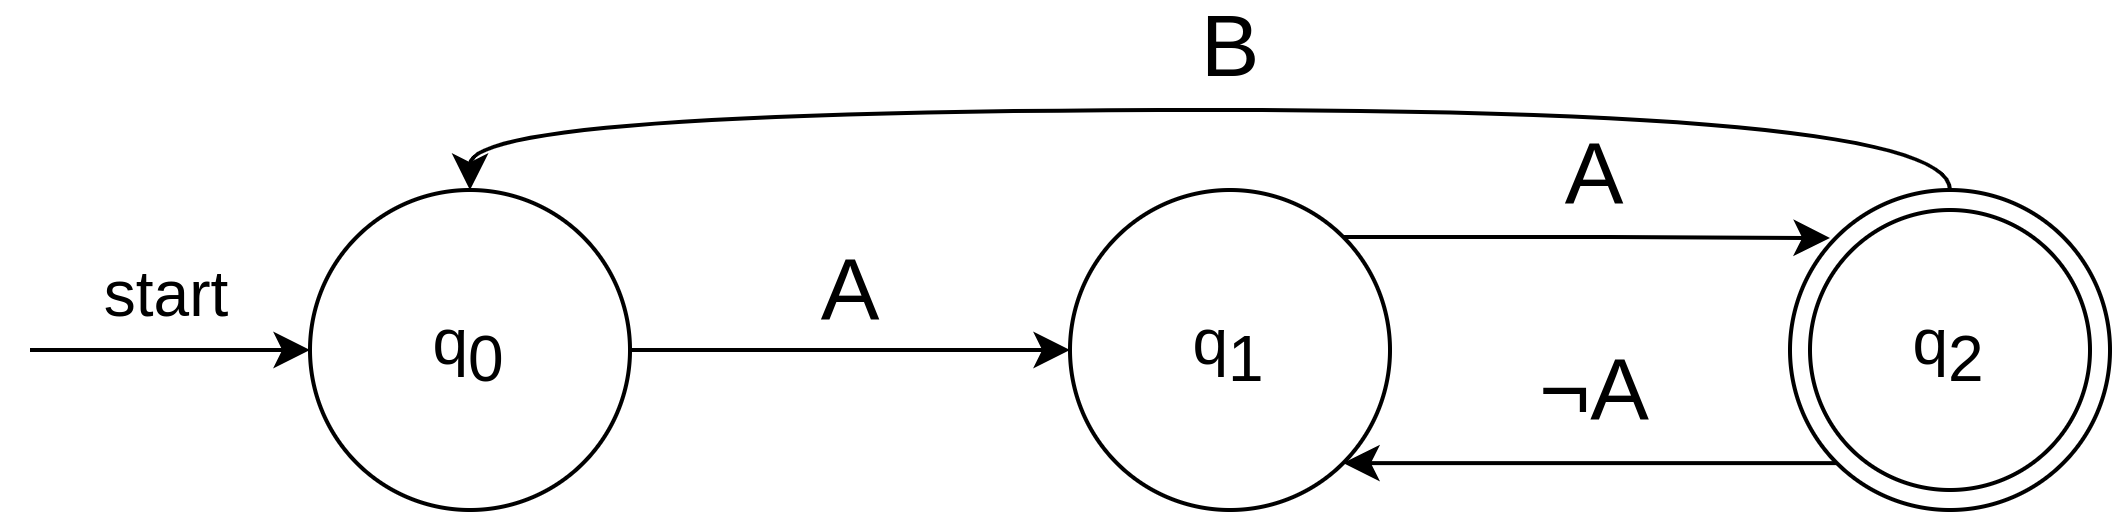
\includegraphics[width=0.8\linewidth]{figures/nba-example.png}
    \caption{Example of NBA accepting any word where every B is preceded by a positive even number of A}
    \label{fig:nba-example}
\end{figure}

There exists a generalization of B{\"u}chi Automata with $n$ acceptance sets of states and the acceptance condition changes as follows: there exists some states that visit each acceptance set of states infinitely many times. It is always possible to compile a Generalized B{\"u}chi Automaton to a Non-deterministic B{\"u}chi Automaton, but GBAs are easier to be used in many cases, like some model checking algorithms.

\begin{definition}[\cite{gastin-oddoux-2001} Generalized B{\"u}chi Automata (GBA)]
A Generalized B{\"u}chi Automata $\automaton$ is a tuple $\automaton = \tuple{\Sigma,Q,I,\delta,\set{F_1,\dots,F_n}}$ where $\Sigma$, $Q$, $I$ and $\delta$ have the same definition of a NBA, but there are $n$ acceptance sets of states $F_1,\dots,F_n$ such that $F_i \subseteq Q$ for all $i \in [1,n]$.
\end{definition}

\begin{definition}[\cite{gastin-oddoux-2001} Run and Language of a GBA]
Let $\automaton = \tuple{\Sigma,Q,I,\sigma,\set{F_1,\dots,F_n}}$ be a GBA and $\sigma = \sequence{\sigma_0,\sigma_1} \in \Sigma^{w}$ be a $\omega$-word over $\Sigma$.
A run of $\automaton$ over $\sigma$ is an infinite sequence of states $\tau = \sequence{q_0,q_1,\dots} \in Q^w$ such that $q_0 \in I$ and $\tuple{q_i,\sigma_i,q_{i+1}} \in \delta$, for each $i \in [0,n]$.
We say that $\tau$ is accepting if and only if for each acceptance set of states $F \in \set{F_1,\dots,F_n}$ there exists a state $q_i \in F$ for infinitely many $i \in \Nat$.
A $\omega$-word $\sigma$ is accepted by $\automaton$ if and only if there exist an accepting run of $\automaton$ over $\sigma$. 
The language accepted by $\automaton$, denoted as $\lang{\automaton}$, is the set of all and only the $\omega$-words $\sigma \in \Sigma^\omega$ accepted by $\automaton$.
\end{definition}

Two important classes of $\omega$-regular languages comprise those languages that express the fact that something bad never happens, called safety languages, and those languages that express that fact that something good eventually happens, called co-safety languages.
The class of the $\omega$-regular co-safety languages coSAFETY is defined as the dual of SAFETY, that is the set of languages $\omegalang{}$ such that $\omegalang{} \in coSAFETY$ iff $\bar{\omegalang{}} \in SAFETY$, where $\bar{\omegalang{}}$ is the complement language of $\omegalang{}$.

\begin{definition}[\cite{geatti-2021-09} Safety languages]
Let $\omegalang{} \subseteq \Sigma^\omega$ be an $\omega$-regular language. We say that $\omegalang{}$ is a safety language if and only if for all words $\sigma \in \Sigma^\omega$ it holds that, if $\sigma \not\in \lang{}$, then $\exists i \in \Nat .\; \forall \sigma' \in \Sigma^\omega .\; \sigma_{[0,i]} \cdot \sigma' \not\in \lang{}$. We call $\sigma_{[0,i]}$ a bad-prefix since it leads to a state where a word can not be in the language no matter how it is going to evolve.
The class of safety $\omega$-regular languages is denoted as SAFETY.
\end{definition}

\begin{definition}[\cite{geatti-2021-09} Co-safety languages]
Let $\omegalang{} \subseteq \Sigma^\omega$ be a $\omega$-regular language. We say that $\omegalang{}$ is a co-safety language if and only if for all words $\sigma \in \Sigma^\omega$ it holds that, if $\sigma \in \lang{}$, then $\exists i \in \Nat .\; \forall \sigma' \in \Sigma^\omega .\; \sigma_{[0,i]} \cdot \sigma' \in \lang{}$. We call $\sigma_{[0,i]}$ a good-prefix since it leads to a state where a word is in the language no matter how it is going to evolve.
The class of co-safety $\omega$-regular languages is denoted as coSAFETY.
\end{definition}

Since each $\omega$-regular language is recognized by a NBA, it is easy to see that we could categorize all automata accepting safety languages. This type of automata is called Safety Automata and are used a lot in my thesis, so let me state them.

\begin{definition}[\cite{gastin-oddoux-2001} Safety Automata (NSA and DSA)]
A Non-deterministic Safety Automata is a tuple $\automaton = \tuple{\Sigma,Q,I,\delta}$, where: (i) $\Sigma$ is a finite alphabet; (ii) $Q$ is a finite set of states; (iii) $I \subseteq Q$ is the set of initial states; (iv) $\delta \subseteq Q \times \Sigma \times Q$ is the transition relation.
If $\delta$ is a partial function $\delta \colon Q \times \Sigma \to Q$, we say that $\automaton$ is a Deterministic Safety Automata (NSA). 
\end{definition}

\begin{definition}[\cite{gastin-oddoux-2001} Run and Language of a NSA]
Let $\automaton = \tuple{\Sigma,Q,I,\sigma}$ be a NSA and $\sigma = \sequence{\sigma_0,\sigma_1} \in \Sigma^{w}$ be a $\omega$-word over $\Sigma$.
A run of $\automaton$ over $\sigma$ is an infinite sequence of states $\tau = \sequence{q_0,q_1,\dots} \in Q^w$ such that $q_0 \in I$ and $\tuple{q_i,\sigma_i,q_{i+1}} \in \delta$, for each $i \in [0,n]$.
A $\omega$-word $\sigma$ is accepted by $\automaton$ if and only if there exist a run of $\automaton$ over $\sigma$. 
The language accepted by $\automaton$, denoted as $\omegalang{(\automaton)}$, is the set of all and only the $\omega$-words $\sigma \in \Sigma^\omega$ accepted by $\automaton$.
\end{definition}

It is simple to see that the language recognized by any safety automaton is a safety language, since the only way for a $\omega$-word to be rejected by a safety automaton is to induce a run that at some point gets stuck, i.e. it can not continue to any state reading the current letter. This implies that a $\omega$-word rejected by a safety automaton is rejected in a finite number of steps, inducing a bad-prefix.  

\begin{theorem}
Given $\omegalang{}$ a language over infinite words, $\omegalang{} \in SAFETY$ if and only if $\omegalang{}$ is recognized by some NSA.
\end{theorem}
